\subsubsection{Domain specific features}
\label{sec:methods_features_domain}

The objective of including domain specific features is to add into the
secondary model data that is intrinsically representative of the underlying
technology and market behavior. This subsection shows and explains the
transformations incurred to the listed features in \ref{sec:material_data_bitcoin_features}.

\paragraph{Addresses:} this group is composed of: \emph{total-addresses},
\emph{new-addresses}, \emph{active-addresses}, \emph{total-addresses},
\emph{sending-addresses}, \emph{receiving-addresses}. We can split these
features into two groups, in figure \ref{fig:total_addresses} the evolution of
total registered addresses in the network is plotted. A logarithm transformation
is show as well in green to stabilize its variance and range. Then, in figure
\ref{fig:addresses} we see the evolution of the other features. The reader may
observe the strong correlation between these four indexes and validate the
observation by inspecting figure \ref{fig:addresses_correlation} which shows the
correlation matrix between these four attributes. Because of that, only
\emph{active-addresses} will be used to train the model. We computed the
fractional differentiation optimum $d$ value for the latter index and turned out
to be 0.1. 

\begin{figure}[H]
    \centering
    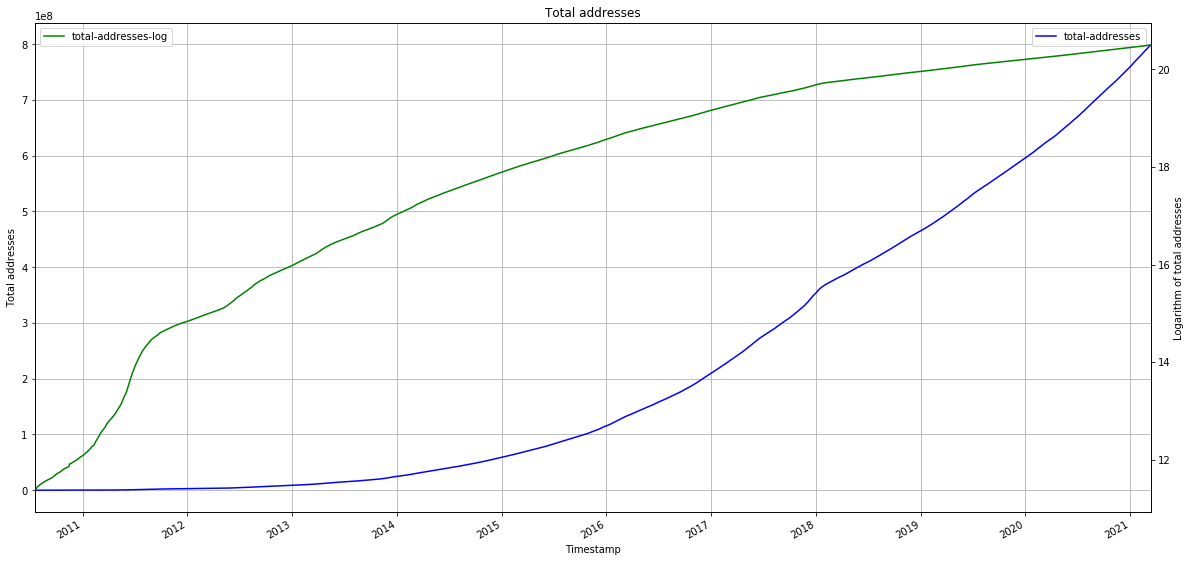
\includegraphics[width=\textwidth]{methods/images/total_addresses.png}
    \caption{Evolution of total registered addresses over time.}
    \label{fig:total_addresses}
\end{figure}

\begin{figure}[H]
    \centering
    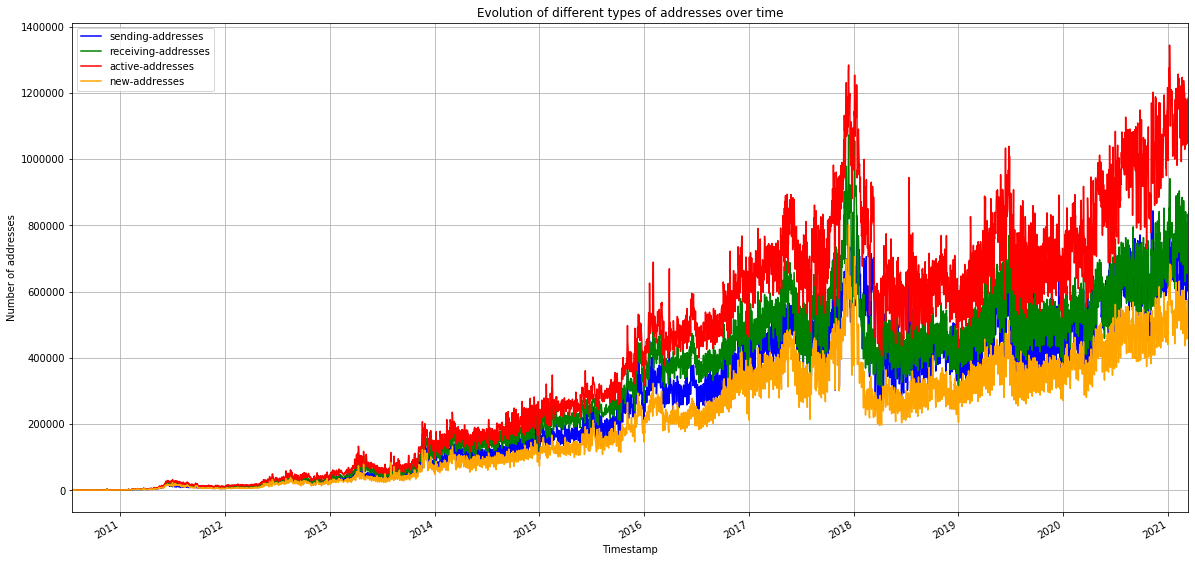
\includegraphics[width=\textwidth]{methods/images/addresses.png}
    \caption{Evolution of \emph{new-addresses}, \emph{active-addresses}, \emph{total-addresses},
\emph{sending-addresses} and \emph{receiving-addresses} over time.}
    \label{fig:addresses}
\end{figure}

\begin{figure}[H]
    \centering
    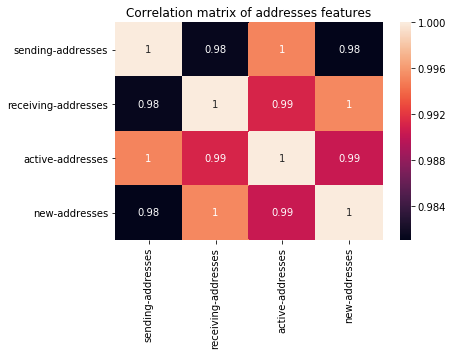
\includegraphics[width=0.7\textwidth]{methods/images/addresses_correlation_mat.png}
    \caption{Correlation matrix of \emph{new-addresses}, \emph{active-addresses}, \emph{total-addresses},
\emph{sending-addresses} and \emph{receiving-addresses}.}
    \label{fig:addresses_correlation}
\end{figure}

\paragraph{Blocks:} in this group There are: \emph{blocks-mined},
\emph{block-interval-mean}, \emph{block-interval-median}, \emph{block-size-mean}
and \emph{block-size-total}. The first three exhibit a quite similar tendency
(see figure \ref{fig:blocks_produced_blocks_mined}) which is aligned with what
they mean: \emph{blocks-mined} describes the number of blocks added to the
blockchain and the other two are centrality measures of the production rate. The
correlation matrix confirms it, see figure \ref{fig:blocks_production_blocks_mined_corr}.
Only \emph{blocks-mined} will be used to avoid adding redundant information.
On the other hand, we have the \emph{block-size-mean} and
\emph{block-size-total} which are expressed in bytes. Both indexes are expected
to be correlated and \ref{fig:block_size} shows their evolution over time. A
fractional differentiation transformation is not enough to stabilize the series
and a logarithmic transformation is applied which results in
\ref{fig:block_size_log}. Only the logarithm of \emph{block-size-total} will be
used to train the model between these two.

\begin{figure}[H]
    \centering
    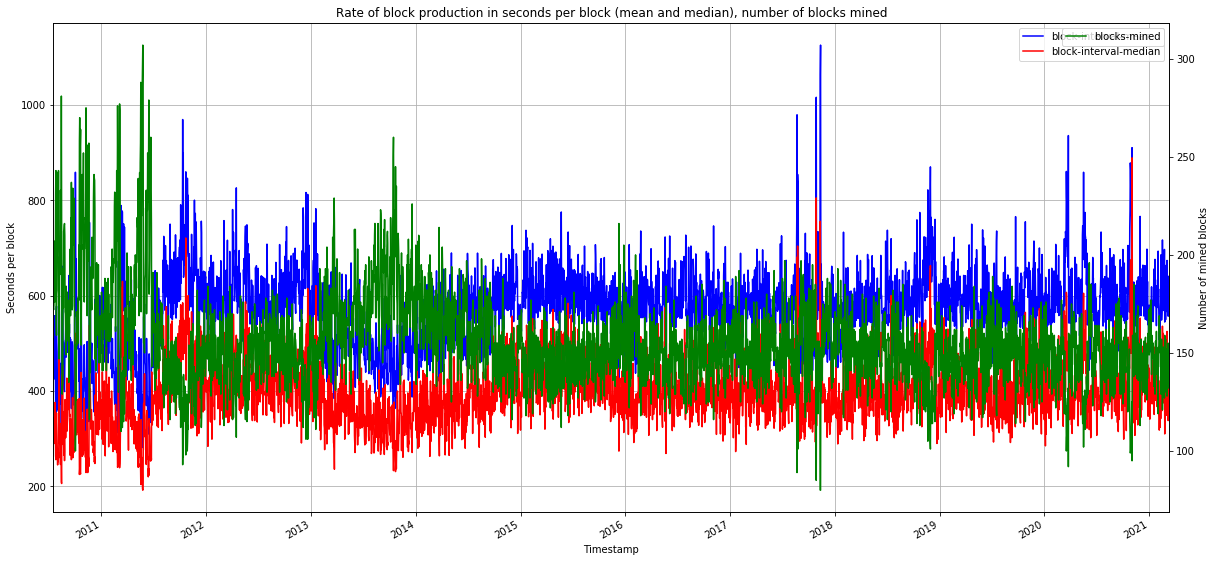
\includegraphics[width=\textwidth]{methods/images/block_production_blocks_mined.png}
    \caption{Evolution of \emph{block-interval-mean} and \emph{block-interval-median} are tracked on the left y-axis. \emph{blocks-mined} is tracked on the right y-axis.}
    \label{fig:blocks_produced_blocks_mined}
\end{figure}

\begin{figure}[H]
    \centering
    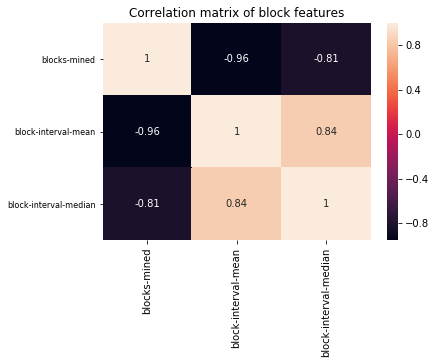
\includegraphics[width=0.7\textwidth]{methods/images/block_production_blocks_mined_corr.png}
    \caption{Correlation matrix of \emph{blocks-mined}, \emph{block-interval-mean} and \emph{block-interval-median}.}
    \label{fig:blocks_production_blocks_mined_corr}
\end{figure}

\begin{figure}[H]
    \centering
    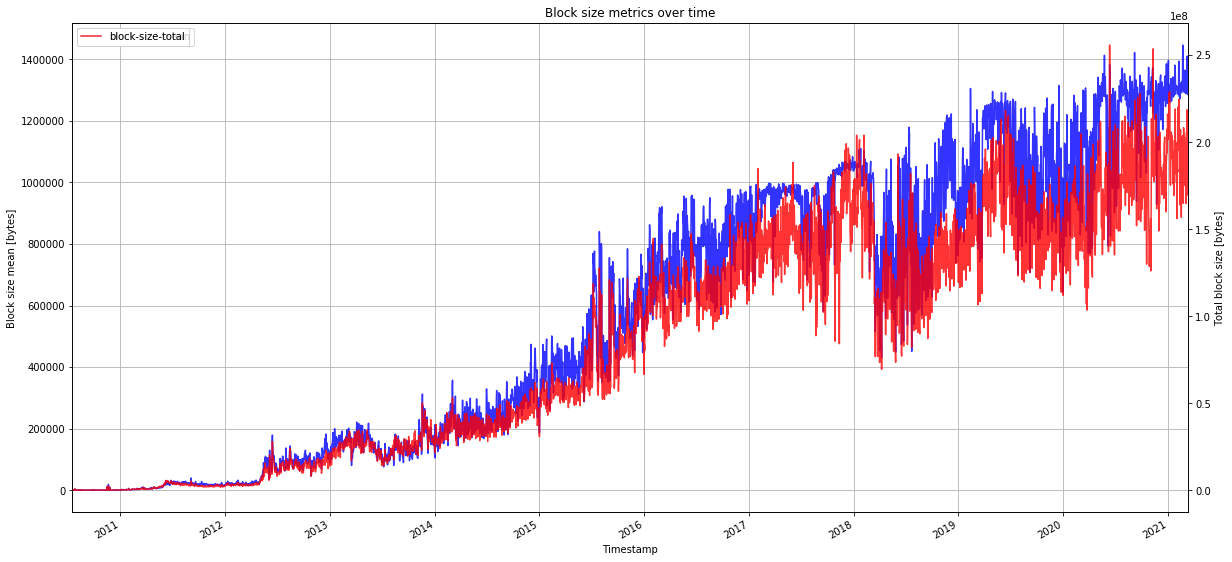
\includegraphics[width=\textwidth]{methods/images/block_size.png}
    \caption{Evolution of \emph{block-size-mean} (in blue and tracked on the left y axis) and \emph{block-size-total} (in red and tracked on the right y axis) over time.}
    \label{fig:block_size}
\end{figure}

\begin{figure}[H]
    \centering
    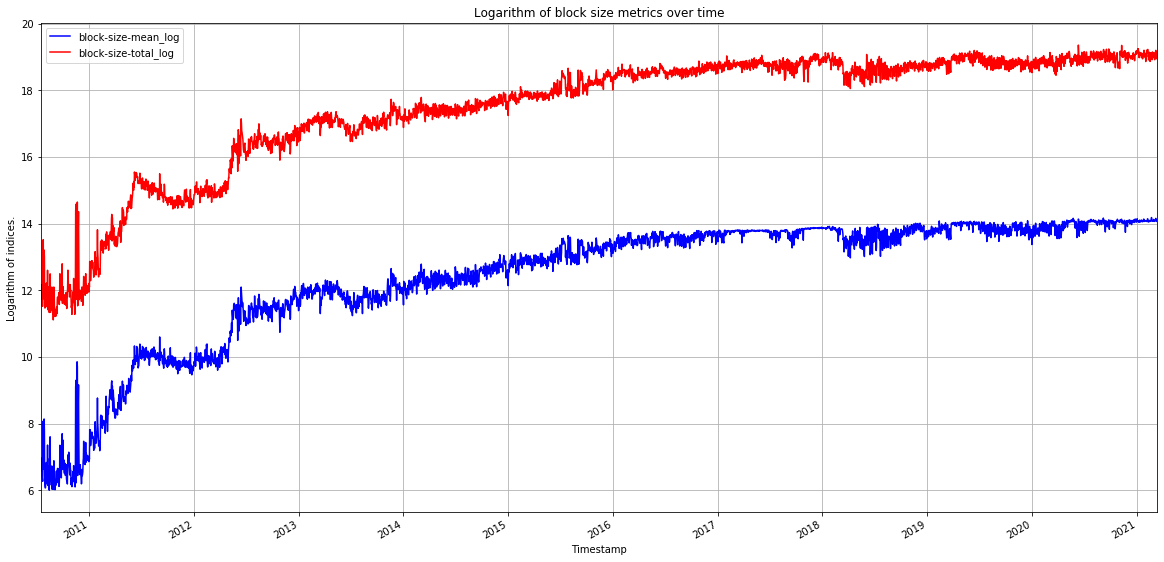
\includegraphics[width=\textwidth]{methods/images/block_size_log.png}
    \caption{Same features as in \ref{fig:block_size} but with a logarithmic transformation. Due to the change of scale, both features are tracked on the same left y axis.}
    \label{fig:block_size_log}
\end{figure}

\paragraph{Fees:} there are two features related to fees: \emph{fees-total} and
\emph{fees-mean}. They both remain relatively stable with very low values but 
there are high valued outliers that get out of range rapidly. Fractional
differentiation was tried but ended up in very low values of $d$ that made no
significant change.  A logarithmic transformation is applied to account the explosive change in local variance when
these outliers occur. Note also that because some values in the series are zero,
a $1$ is added to the logarithm argument to avoid having minus infinity in the
series after the transformation. For illustration purposes, figure
\ref{fig:total_fees} is shown.

\begin{figure}[H]
    \centering
    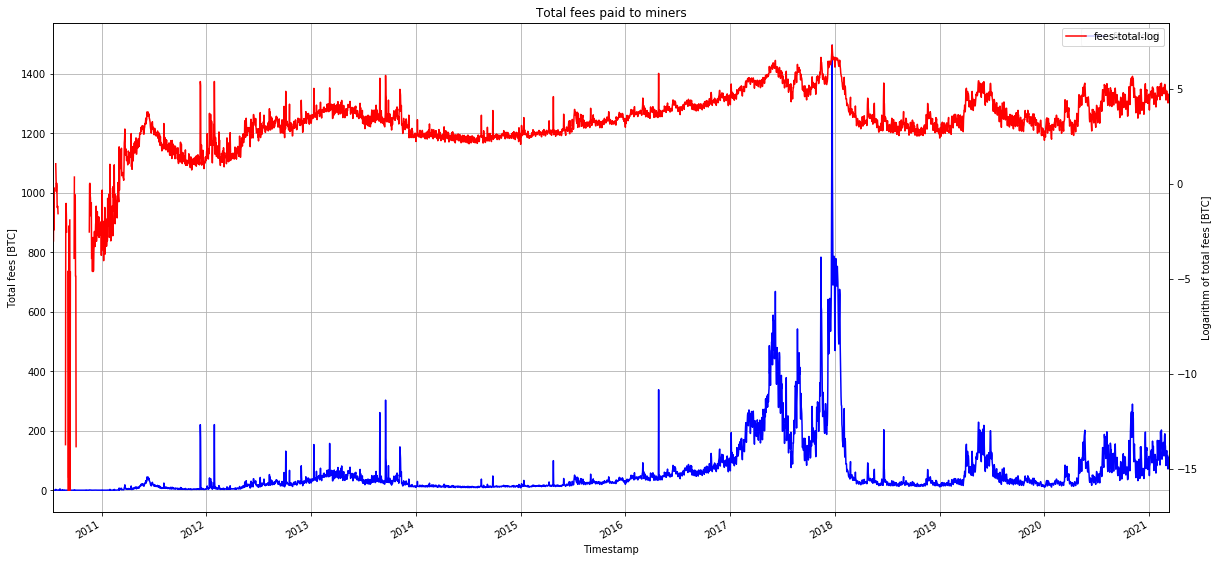
\includegraphics[width=\textwidth]{methods/images/total_fees.png}
    \caption{Evolution of \emph{fees-total} (in blue) and its the logarithmic transformation (in red) over time. The left y axis tracks the linear scale and the right y axis tracks the logarithmic scale.}
    \label{fig:total_fees}
\end{figure}

\paragraph{General indicators:} in this group we have \emph{sopr}, \emph{ratio},
\emph{daysTillHalving}, \emph{price-drawdown-from-ath}, \emph{market-cap} and
\emph{circulating-supply}. The relationship between \emph{market-cap} and 
\emph{ratio} was already explained in section \ref{sec:intro_domain} when
referring to the stock to flow model so it will be omitted in this case. We will
just mention that \emph{market-cap} will suffer a logarithmic transformation to
stabilize its range. \emph{sopr} and \emph{price-drawdown-from-ath} are indexes
so no further transformation is required (see figures \ref{fig:sopr} and
\ref{fig:price-drawdown-from-ath}). Moreover, the \emph{circulating-supply}
values are in the order of millions and evolves asymptotically to 18 millions as
the issuance model expects it to be. In particular, we will create a derivative
index from the supply computed as the differentiated series of circulating
supply logarithm which shows the speed of issuance (see figure \ref{fig:circulating_supply_rate}).

\begin{figure}[H]
    \centering
    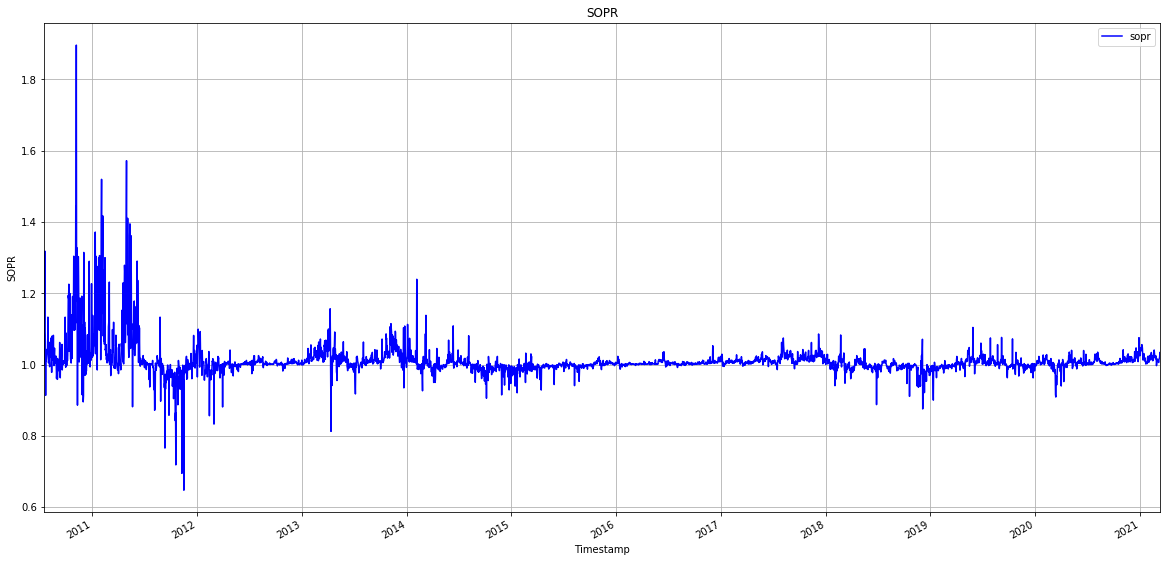
\includegraphics[width=\textwidth]{methods/images/sopr.png}
    \caption{Evolution of \emph{sopr} over time.}
    \label{fig:sopr}
\end{figure}

\begin{figure}[H]
    \centering
    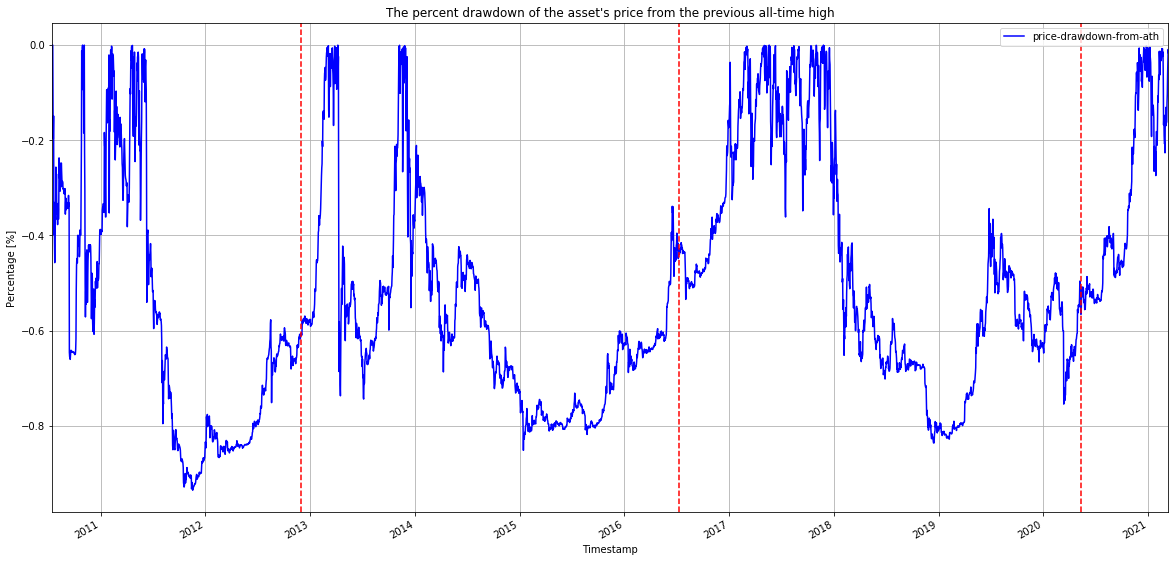
\includegraphics[width=\textwidth]{methods/images/price-drawdown-from-ath.png}
    \caption{Evolution of \emph{price-drawdown-from-ath} over time. In vertical
    dashed red lines the halving dates are displayed}
    \label{fig:price-drawdown-from-ath}
\end{figure}

\begin{figure}[H]
    \centering
    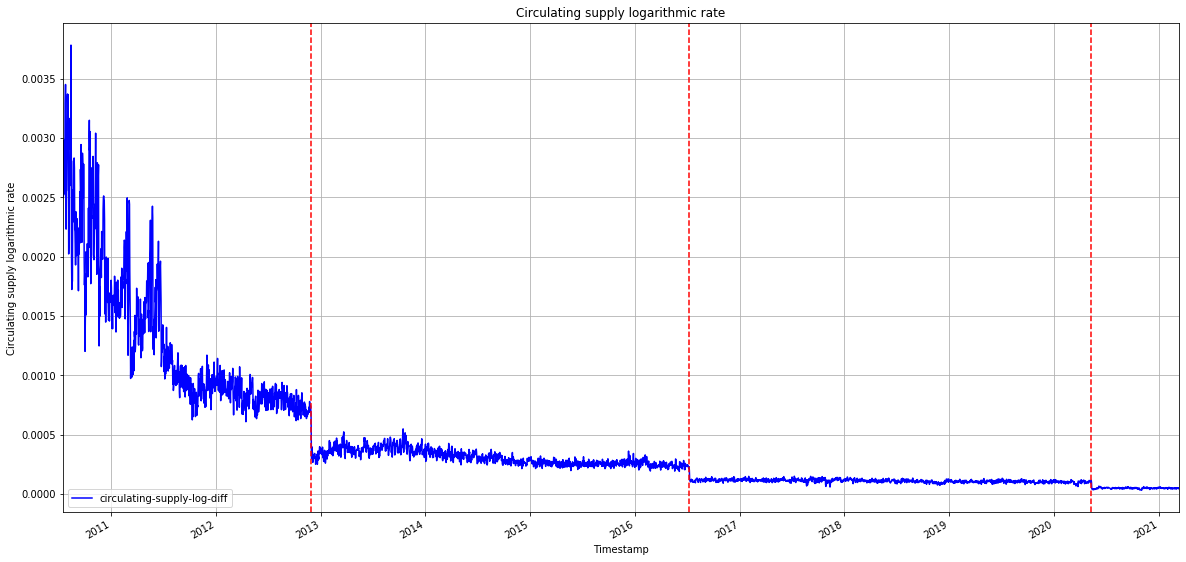
\includegraphics[width=\textwidth]{methods/images/circulating_supply_rate.png}
    \caption{Evolution of the logarithm of issuance over time. In vertical
    dashed red lines the halving dates are displayed.}
    \label{fig:circulating_supply_rate}
\end{figure}


\paragraph{Transactions:} in this group we have \emph{transaction-size-total},
\emph{transaction-rate}, \emph{transaction-count}, \emph{transaction-size-mean},
\emph{transfer-volume-mean} and \emph{transfer-volume-median}. As it can be seen
in figure \ref{fig:transaction_corr}, the three indexes
\emph{transaction-size-total}, \emph{transaction-rate}, and 
\emph{transaction-count} are highly correlated so only one will be taken as
input to the model, in particular the \emph{transaction-rate}. A note about this
index can be done when looking at the histogram which seems to be bimodal. A
derivative index is created from it which groups the values into their deciles
and aims to reduce the high frequency changes in the transaction rate that
affect the signal on a daily basis. Figure \ref{fig:transaction_rate} shows it
in detail. Moving to \emph{transaction-size-mean} the index exhibits some
frequent spikes but those are within range and there is no clear trend so the
feature remains as is (\ref{fig:transaction_size_mean}). Central transfer volume
features (\emph{transfer-volume-mean} and \emph{transfer-volume-median}) exhibit
a high volatility in the first issuance period and then it is more and more
stable. A logarithmic transformation is applied to both and even though they
try to predict the same, their tendencies are different in values and capture
differently the local volatility so both will be preserved (
\ref{fig:transfer_volume_central}). Similarly to the processing done to the
others, the \emph{transfer-volume-total} is transformed with a logarithm (
\ref{fig:transfer-volume-total}).

\begin{figure}[H]
    \centering
    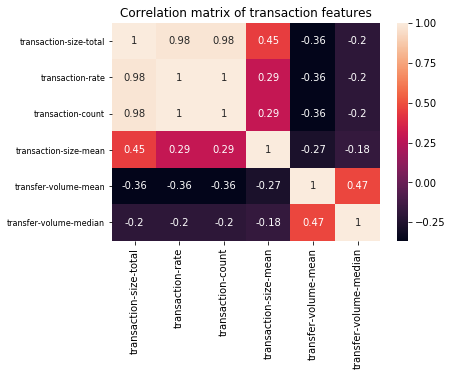
\includegraphics[width=0.7\textwidth]{methods/images/transaction_corr.png}
    \caption{Correlation matrix between the transaction related features}
    \label{fig:transaction_corr}
\end{figure}

\begin{figure}[H]
    \centering
    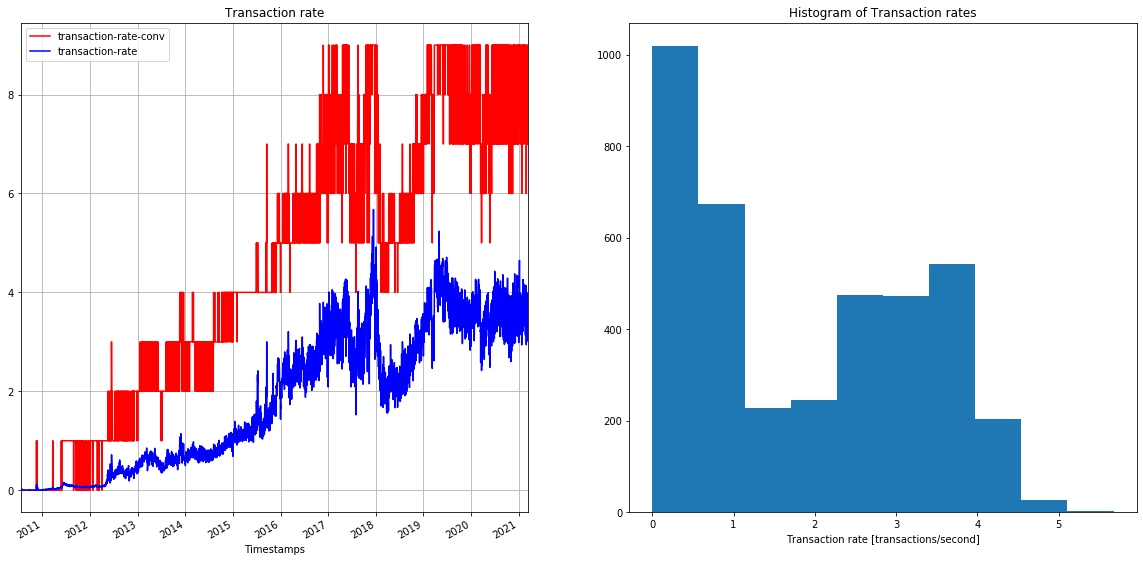
\includegraphics[width=\textwidth]{methods/images/transaction_rate.png}
    \caption{Left: \emph{transaction-rate} (in blue) and decile index of the same feature (in red) over time. Right: histogram of \emph{transaction-rate}.}
    \label{fig:transaction_rate}
\end{figure}

\begin{figure}[H]
    \centering
    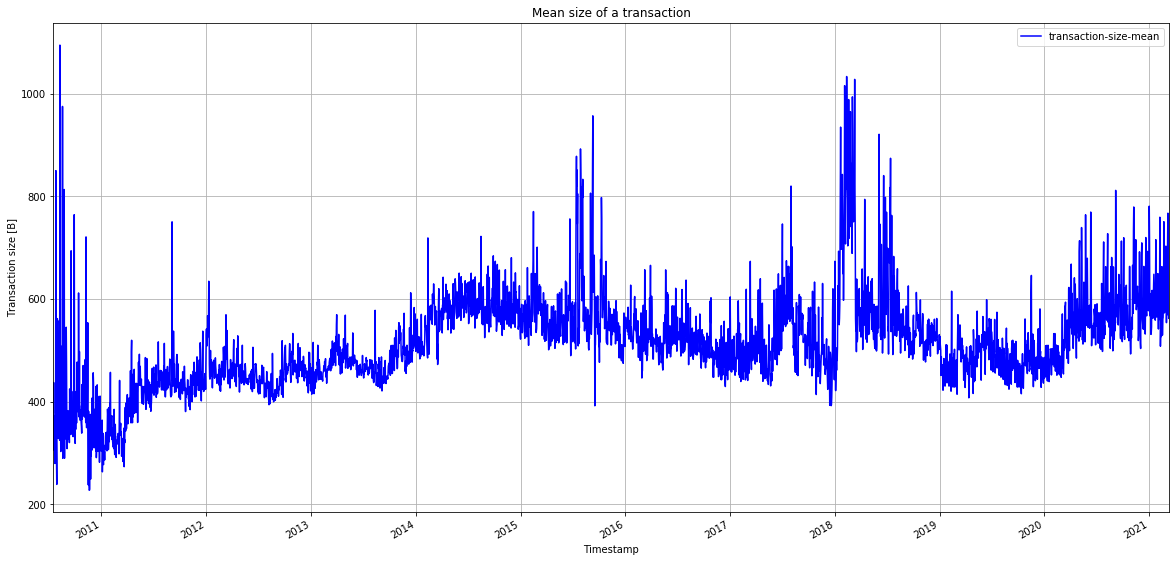
\includegraphics[width=\textwidth]{methods/images/transaction_mean_size.png}
    \caption{Evolution of \emph{transaction-size-mean} over time.}
    \label{fig:transaction_size_mean}
\end{figure}

\begin{figure}[H]
    \centering
    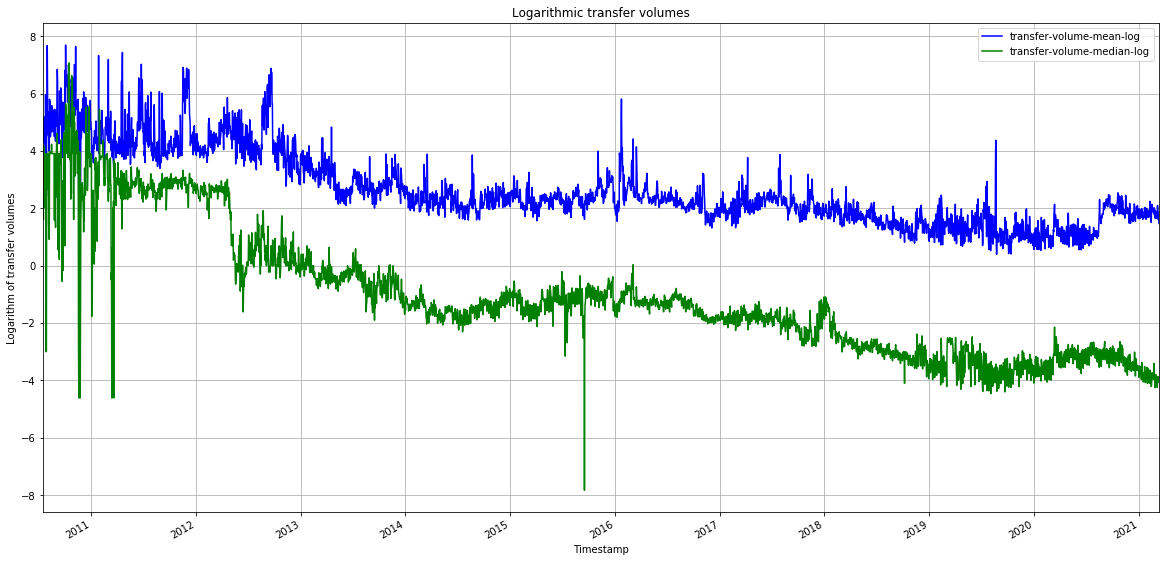
\includegraphics[width=\textwidth]{methods/images/transfer_volume_central.png}
    \caption{Evolution of the logarithm of \emph{transfer-volume-mean} and \emph{transfer-volume-median}.}
    \label{fig:transfer_volume_central}
\end{figure}

\begin{figure}[H]
    \centering
    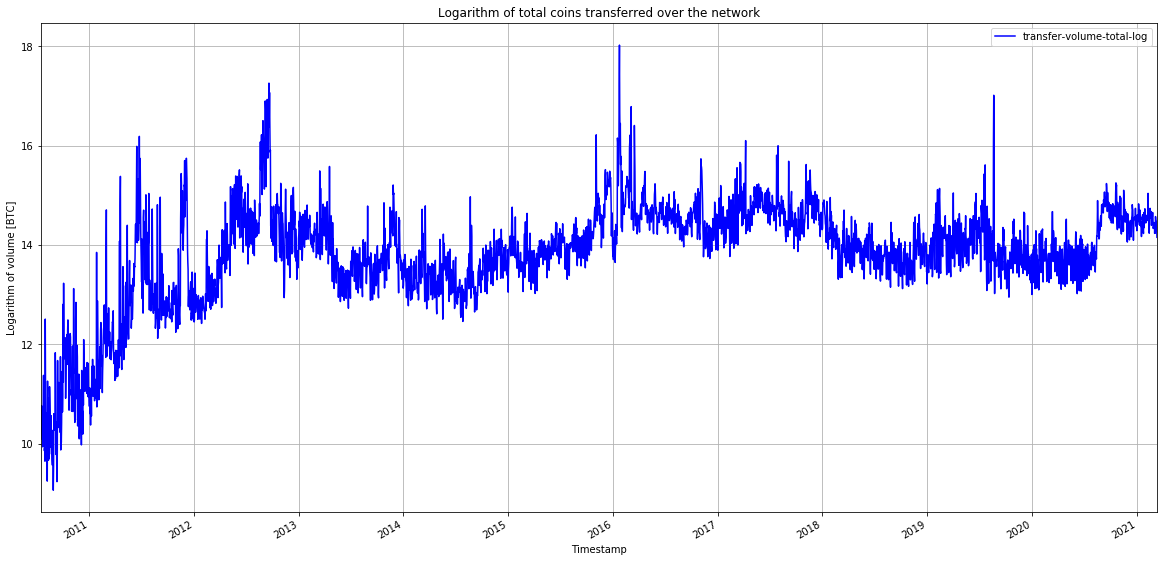
\includegraphics[width=\textwidth]{methods/images/transfer_volume_total.png}
    \caption{Evolution of the logarithm of \emph{transfer-volume-total} over time.}
    \label{fig:transfer-volume-total}
\end{figure}

\paragraph{Unspent / spent transactions:} under this final group we can find:
\emph{utx-os-created} \emph{utx-os-spent}, \emph{utxo-value-spent-mean},
\emph{utxo-value-spent-median} and \emph{utxo-value-created-mean}. Following the
same procedure as with the others, a correlation matrix between these features
is created and shown in figure \ref{fig:utxo_corr}. We can find two pairs of
highly correlated features: \emph{utx-os-created} with \emph{utx-os-spent}, and
\emph{utxo-value-created-mean} with \emph{utxo-value-spent-mean}. Note that
\emph{utxo-value-spent-median} is mildly correlated with the others (0.48 and
0.49 respectively) which makes this feature to be kept. Provided that
\emph{utx-os-created} is a super set of \emph{utx-os-spent}, the former will be
preferred (see figure \ref{fig:utxo_created}). The same reasoning applies to
 \emph{utxo-value-created-mean} (see figure \ref{fig:mean_utxo_created}).



\begin{figure}[H]
    \centering
    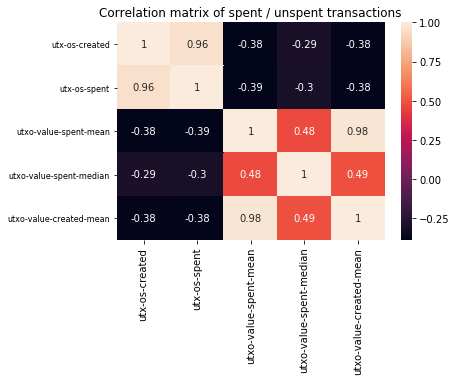
\includegraphics[width=0.7\textwidth]{methods/images/utxo_corr.png}
    \caption{Correlation matrix between unspent / spent transaction features.}
    \label{fig:utxo_corr}
\end{figure}

\begin{figure}[H]
    \centering
    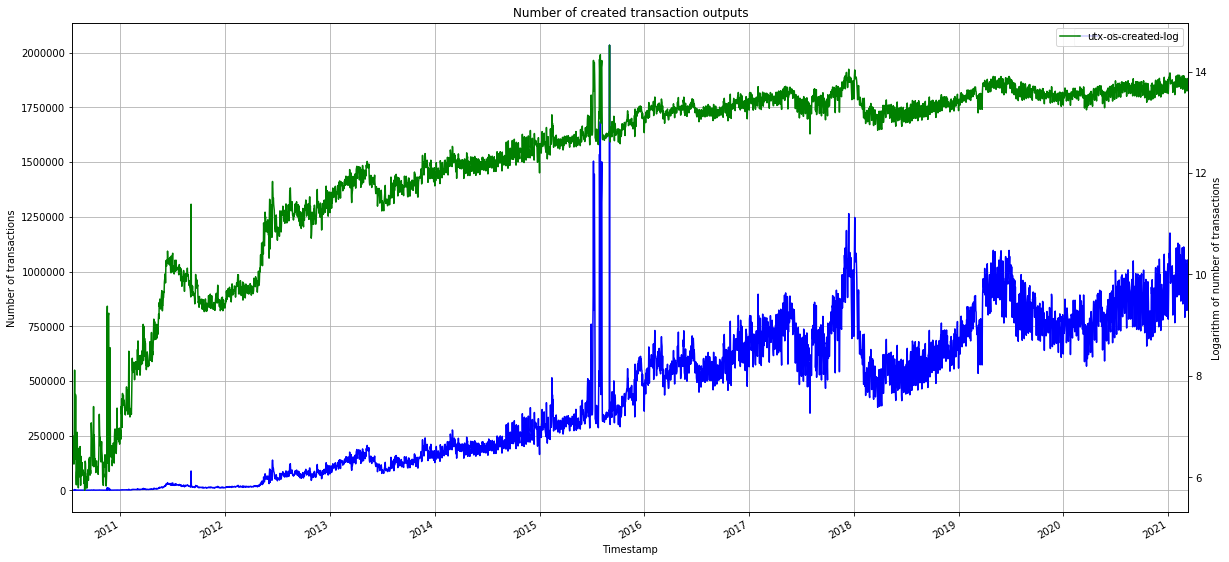
\includegraphics[width=\textwidth]{methods/images/utxo_created.png}
    \caption{Evolution \emph{utx-os-created} (in blue) and its logarithmic transform (in green) over time.}
    \label{fig:utxo_created}
\end{figure}

\begin{figure}[H]
    \centering
    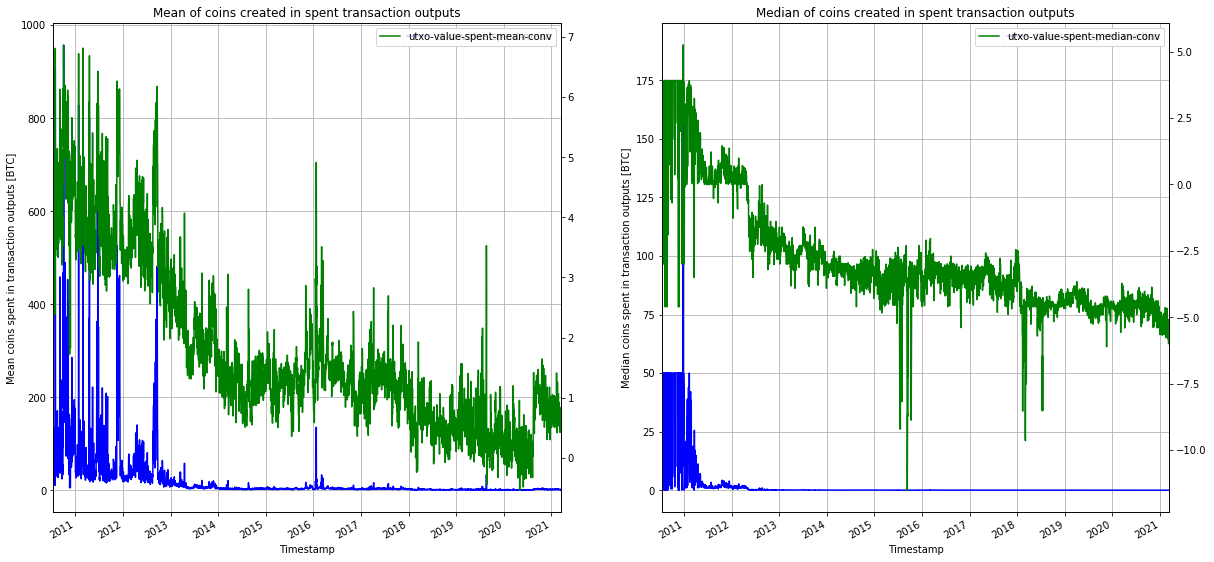
\includegraphics[width=\textwidth]{methods/images/utxo_value_spent.png}
    \caption{Left: evolution of \emph{utxo-value-created-mean} (blue) and its logarithmic transformation (in green) over time. Right: evolution of \emph{utxo-value-created-median} (blue) and its logarithmic transformation (in green) over time.}
    \label{fig:utxo_value_spent}
\end{figure}

\begin{figure}[H]
    \centering
    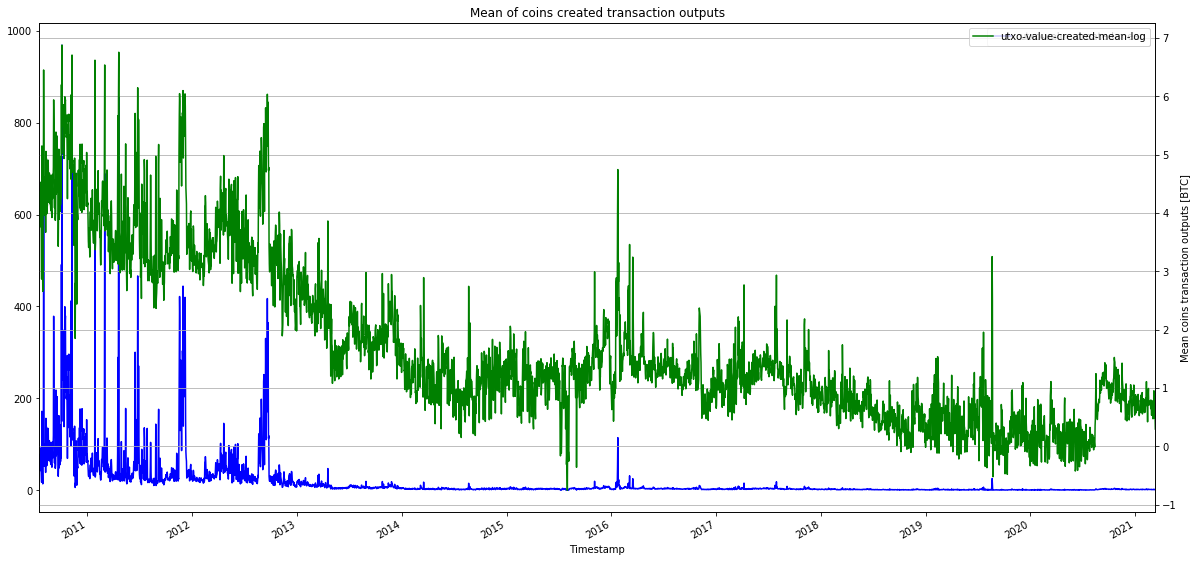
\includegraphics[width=\textwidth]{methods/images/mean_utxo_created.png}
    \caption{Evolution of \emph{utxo-value-created-mean} (in blue) and its logarithmic transformation (in green) over time.}
    \label{fig:mean_utxo_created}
\end{figure}